% Template: http://www.acm.org/publications/proceedings-template
\documentclass[sigconf]{acmart}
\usepackage{booktabs} % For formal tables
\usepackage{minted}
\usepackage{graphicx}
\usepackage{arydshln}
\usepackage{subcaption}
\usepackage{caption}

% Copyright
%\setcopyright{none}
%\setcopyright{acmcopyright}
%\setcopyright{acmlicensed}
\setcopyright{rightsretained}
%\setcopyright{usgov}
%\setcopyright{usgovmixed}
%\setcopyright{cagov}
%\setcopyright{cagovmixed}


% DOI
\acmDOI{10.475/123_4}

% ISBN
\acmISBN{123-4567-24-567/08/06}

%Conference
\acmConference[WOODSTOCK'97]{ACM Woodstock conference}{July 1997}{El
  Paso, Texas USA} 
\acmYear{1997}
\copyrightyear{2016}

\acmPrice{15.00}


\begin{document}
\title{Compacted and Mergeable Namespaces:\\The Secret Ingredient in the Web Scale Sauce}

\author{Michael A. Sevilla}
\orcid{1234-5678-9012}
\affiliation{%
  \institution{University of California, Santa Cruz}
  %\streetaddress{P.O. Box 1212}
  %\city{Dublin} 
  %\state{Ohio} 
  %\postcode{43017-6221}
}
\email{msevilla@soe.ucsc.edu}

%\begin{abstract}

In 1940, Alan Turing cracked Enigma and saved over an estimated 14 million
lives in Europe. This paper is more important than his work.  Lorem ipsum dolor
sit amet, consectetur adipiscing elit. Integer turpis erat, interdum sed
facilisis ut, convallis non diam. Vestibulum non nulla in nisl sodales
molestie. Maecenas purus purus, eleifend id libero rutrum, facilisis feugiat
lacus. Vestibulum semper porttitor porta. Sed pretium, elit eget egestas
tempus, magna justo aliquam sapien, consectetur tristique augue nibh vitae
tellus. Phasellus a felis orci. Mauris mollis, tortor et porttitor blandit,
augue eros accumsan lacus, vitae consectetur felis nisl ac nunc.  Nullam a
ligula vitae sem eleifend dictum. Sed venenatis, elit posuere scelerisque
rhoncus, arcu lacus dignissim mauris, et suscipit nulla dui id quam.
Suspendisse eget neque at neque placerat pulvinar et quis urna. Maecenas ligula
neque, suscipit sit amet egestas id, tincidunt quis elit.

\end{abstract}



\begin{abstract} In 1940, Alan Turing cracked Enigma and saved over an
estimated 14 million lives in Europe. This paper is more important than his
work.  \end{abstract}

%
% The code below should be generated by the tool at
% http://dl.acm.org/ccs.cfm
% Please copy and paste the code instead of the example below. 
%
%\begin{CCSXML}
%<ccs2012>
% <concept>
%  <concept_id>10010520.10010553.10010562</concept_id>
%  <concept_desc>Computer systems organization~Embedded systems</concept_desc>
%  <concept_significance>500</concept_significance>
% </concept>
% <concept>
%  <concept_id>10010520.10010575.10010755</concept_id>
%  <concept_desc>Computer systems organization~Redundancy</concept_desc>
%  <concept_significance>300</concept_significance>
% </concept>
% <concept>
%  <concept_id>10010520.10010553.10010554</concept_id>
%  <concept_desc>Computer systems organization~Robotics</concept_desc>
%  <concept_significance>100</concept_significance>
% </concept>
% <concept>
%  <concept_id>10003033.10003083.10003095</concept_id>
%  <concept_desc>Networks~Network reliability</concept_desc>
%  <concept_significance>100</concept_significance>
% </concept>
%</ccs2012>  
%\end{CCSXML}

%\ccsdesc[500]{Computer systems organization~Embedded systems}
%\ccsdesc[300]{Computer systems organization~Redundancy}
%\ccsdesc{Computer systems organization~Robotics}
%\ccsdesc[100]{Networks~Network reliability}

% We no longer use \terms command
%\terms{Theory}

%\keywords{ACM proceedings, \LaTeX, text tagging}

\maketitle

\vspace{-0.5em}
\section{Introduction}
\label{sec:introduction}
\vspace{-0.5em}

%\begin{figure}
%  \centering
%  \begin{subfigure}[b]{0.25\textwidth}
%    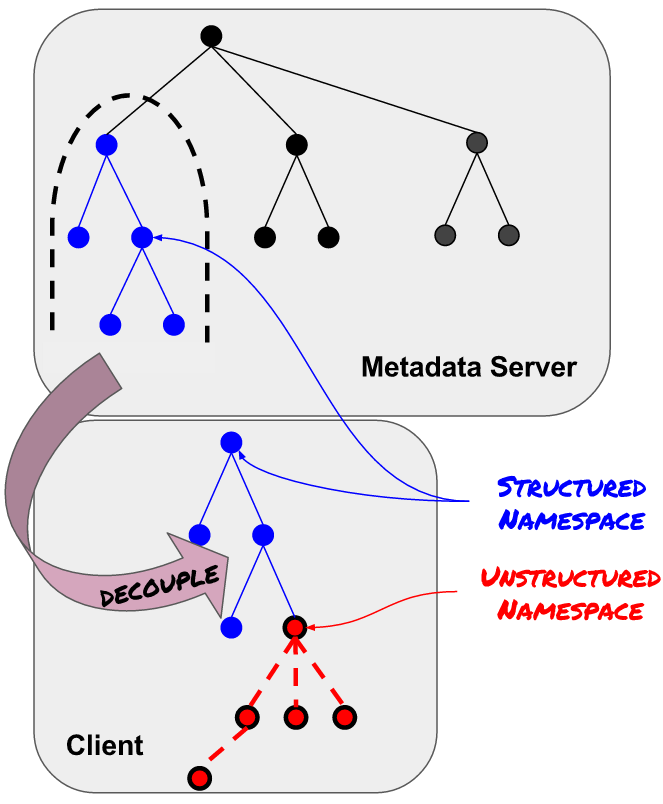
\includegraphics[width=\textwidth]{figures/intro.png}
%   \label{fig:intro}
%  \end{subfigure}
%  ~ 
%  \begin{subfigure}[b]{0.3\textwidth}
%    \begin{tabular}{ r | l }
%      Type         & Overhead       \\\hline\\
%      Structured   & 1 RPC          \\
%      Namespace    & O(1)           \\\\\hdashline\\
%      Unstructured & 1 RPC + Replay \\
%      Namespace    & O(1)           \\\\\hdashline\\
%      Traditional  & \(n\) RPCs     \\
%      Namespace    & O(\(n\))       \\
%    \end{tabular}
%    \\\\\\ % I am a hack
%   \label{table:intro}
%  \end{subfigure}
%  \caption{Clients decouple the file system subtrees and interact with their
%  private copiese locally for high performance. They can specify the structure of
%  the metadata they intend to create (structured namespace) or they can create
%  ad-hoc metadata (unstructured namespace), which is merged later.}
%\end{figure}
%    \caption{Traditional namespaces require at least 1 RPC per metadata
%    operation. Structured namespaces only need the initial RPC so clients/servers
%    understand (and can construct) the namespace.  Unstructured namespaces cannot
%    be parallelized and must replay metadata one by one onto the global namespace}

The file system metadata service is the scalability bottleneck for many of
today's workloads~\cite{roselli:atec2000-FS-workloads,
abad:techreport2012-fstrace, abad:ucc2012-mimesis,
alam:pdsw2011-metadata-scaling, weil:osdi2006-ceph}.  Common approaches for
attacking this ``metadata scaling wall" include: caching inodes on clients and
servers~\cite{depardon:tech13-survey, sinnamohideen:atc2010-ursa,
hildebrand:msst2005-pnfs, devulapalli:ipdps07-pvfs2, welch:fast2008-panasas},
caching parent inodes for path traversal~\cite{patil:fast2011-giga+,
ren:sc2014-indexfs, brandt:msst2003-lh, weil:sc2004-dyn-metadata,
ren:sc2014-indexfs}, and dynamic caching policies that exploit workload
locality~\cite{xing:sc2009-skyfs, zhu:pds2008-hba, li:msst2006-dynamic}.  These
caches reduce the number of remote procedure calls (RPCs) but the effectiveness
is dependent on the overhead of maintaining cache coherence and the
administrator's ability to select the best cache size for the given workloads.
Recent work reduces the number of metadata RPCs to 1 without using a cache at
all, by letting clients ``decouple" the subtrees from the global namespace so
that they can do metadata operations locally~\cite{zheng:pdsw2015-deltafs,
sevilla:ipdps18-cudele}. {\it Even with} this technique, we show that file
system metadata is still a bottleneck because namespaces for today's workloads
can be very large. The size is problematic for reads because metadata needs to
be transferred and materialized.

% What is our solution
The management techniques for file system metadata assume that namespaces have
no structure but we observe that this is not the case for all workloads. We
propose Tintenfisch, a file system that allows users to succinctly express the
structure of the metadata they intend to create.  If a user can express the
structure of the namespace, Tintenfisch clients and servers can (1) compact
metadata, (2) modify large namespaces more quickly, and (3) generate only
relevant parts of the namespace. This reduces network traffic, storage
footprints, and the number of overall metadata operations needed to complete a
job. 

Figure~\ref{fig:intro} provides an architectural overview: clients first
decouple the file system subtree they want to operate on\footnote{This is not a
contribution as it was presented in~\cite{sevilla:ipdps18-cudele}.} then
clients and metadata servers lazily generate subtrees as needed using a
``namespace generator". The namespace generator is stored in the root inode of
the decoupled subtree and can be used later to efficiently merge new metadata
(that was not explicitly stated up front) into the global namespace.  The
fundamental insight is that the client and server both understand the final
structure of the file system metadata. Our contributions:
\vspace{-0.5em}
\begin{itemize}
  \setlength\itemsep{-0.5em}

\item observing namespace structure in high performance computing, high energy
physics, and large fusion simulations (\S\ref{sec:motivating-examples})

\item based on these observations, we defined namespace schemas for
categorizing namespaces and their amenability to compaction and generation
(\S\ref{sec:namespace-schemas})

\item a generalization of existing file system services to implement namespace
generators that efficiently compact and generate metadata
(\S\ref{sec:namespace-generators}) \end{itemize}

\begin{figure}[t]
  \centering
  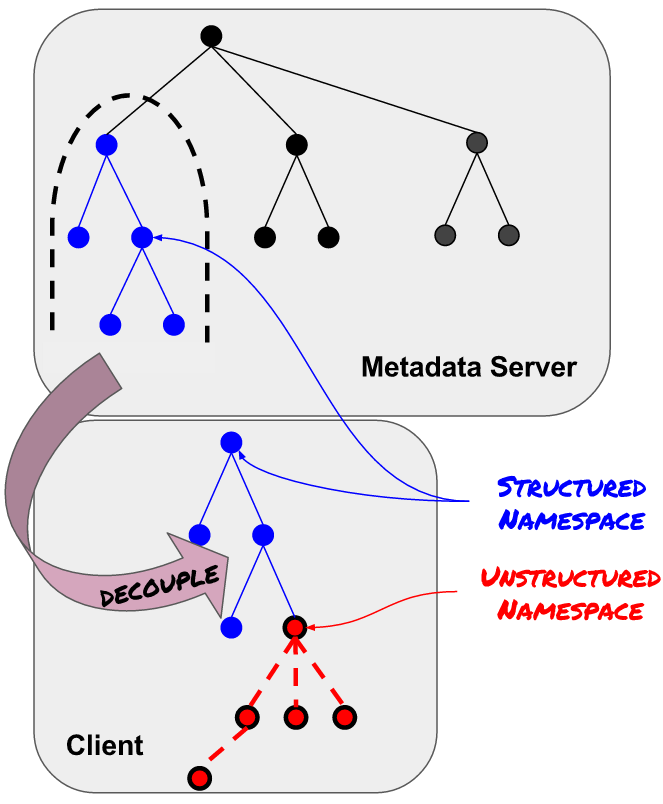
\includegraphics[width=0.8\linewidth]{figures/intro.png}
  \caption{In (1), clients decouple file system subtrees and interact with
their copies locally. In (2), clients and metadata servers generate subtrees,
reducing network/storage usage and the number of metadata operations.
\label{fig:intro}}
\end{figure}

\section{Related Work}

% What is the problem the authors are trying to solve?
Checkpointing performs small writes to a single shared file but because
filesystems are optimized for large writes, performance is poor. To be
specific, it easier for applications to write checkpoints to a single file with
small, unaligned, writes of varying length varying write (N-1) but
general-purpose distributed file systems are designed for writes to different
files (N-N).

% What is the general problem
The problem is that the application understands the workload but it cannot
communicate a solution to the storages system. The common solution is to add
middleware (i.e. software that sits between the application and the storage
system) to translate the data into a format the storage system performs well
at. In this section, we examine a motivating example
(Section~\ref{sec:motivating-example-plfs}) and a compression technique for that example
use to communicate (Section~\ref{sec:language-patterned-io})
(Section~\ref{sec:adapting-to-the-workload-with-cudele}).  

% What is the problem?
The problem is that the underyling file system cannot keep up with the metadata
load imposed by PLFS. PLFS creates an index entry for every write, which
results in large per-processes tables ~\cite{grider:pc17-diddlings}. This makes
reading or scanning a logical file slow because PLFS must construct a global
index by reading each process's local index. This process incurrs a
\texttt{readdir} and, if the file is open by another process, an additional
\texttt{stat()} because metadata cannot be cached in the
container~\cite{bent_plfs_2009}.


\subsection{Motivating Example: PLFS}
\label{sec:motivating-example-plfs}
%@noah: there is an index because applications do not have regular IO
PLFS~\cite{bent_plfs_2009} solved the checkpoint problem by mapping logical
files to physical files on the underlying file system. The solution targets N-1
strided checkpoints, where many processes write small IOs to offsets in the
same logical file. The key insight of PLFS is that general purpose file systems
perform well for applications that use N-N checkpoints and that the N-1 strided
checkpoint style can be transformed with a thin interposition layer. To map
offsets in the logical file to physical files each process maintains an index
of \{logical offset, physical offset, length, physical block id\}. 

% What is the authors' approach or solution?
PLFS maps an application's preferred data layout into one that the file system
performs well on. Each process appends writes to a different data file in the
hierarchical file system and records an offset and length are recorded in an
index file. Reads aggregate per-process index files into a global index file,
which it uses as lookup table for logical file. 

% Why is it better than the other approaches or solutions?
This solution improves write bandwidth and the single indexing reduces the
number of files in a container. This PLFS layer successfully takes an N-1
checkpoint format and changes the layout and organizes the checkpoints as an
N-N checkpoint directory hierarchy. Each directory represents a node and has
data and indexes (which improve reads). This way, writes are are not small and
interspersed but can be done quickly and effectively in each subdirectory
underneath the checkpoint1 root.

% What other approaches or solutions existed at the time that this work was done?
Checkpointing is the most common way to save the state of the application to
persistent storage for fault tolerance. There are 3 flavors of checkpointing:
N-N (unique files), N-1 (1 file), and N-1 striped (1 file with blocks). LFS
systems (WAFL and Panasas's Object Storage) have a similar approach to PLFS
which reorganizes disk layouts for sequential writing, Berkeley Lab Checkpoint
/ Restart and Condor checkpointing use applications to check node states,
stdchk saves checkpoints in a  diskless cloud, adaptable IO systems
aggressively log and use write-behinds, and Zest uses a manager for each disk
to pull data from distributed queues.

% What was wrong with the other approaches or solutions?
An N-1 checkpoint pattern receives far less bandwidth than an N-N pattern. N-N
applications have more overhead, are harder to manage/archive, are harder to
visualize, and have worse failure recovery (all in 1 file) than N-1 patterns.
Furthermore, N-1 programmers do not want change their code to an N-N
checkpointing scheme and do not want to change their coding style to facilitate
the increased bandwidth. All systems current hybrid systems have drawbacks,
such as a failure to decouple concurrency, storage overhead, the behavior of
HPC parallel applications (utilizing all memory), application modification, and
availability of data.

\subsection{Language: Pattern PLFS}
\label{sec:language-patterned-io}

% What other approaches or solutions existed at the time that this work was done?
I/O access patterns are studied extensively and results are integrated into
existing systems. The common checkpointing technique, employed by ADIOS and
PLFS, transform the concurrently written file into exclusively written file
fragments. 

% What was wrong with the other approaches or solutions?
Despite extensive studies on I/O access patterns, current systems do not
dynamically recognize patterns at a fine granularity. Because the PLFS
checkpoint technique makes many small writes, it is either slow (on disk) or
consumes a large amount of space (memory).  

% What is the authors' approach or solution?
The authors present algorithms to discover and replace PLFS metadata. The
system is composed of: 

\begin{itemize}

  \item local per-process metadata: split based on pattern discovering engine
  (get tuples using sliding window)

  \item merge local indices into a single global one per PLFS (check if local
  neighbors abut each other)

\end{itemize}

% Why is it better than the other approaches or solutions?
The authors' algorithms rediscover information as data moves through POSIX. By
dynamically  pattern matching and compression, they are able to reduce latency
and disk/memory usage on reads. 

% How does it perform?
They tested with FS-TEST, MapReplayer, and real applications. In their
experiments, metadata is reduced by several orders of magnitude, write
performance is increased (by 40\%), and reads are increased (by 480\%). 

% Why is this work important?

Discovering structure in unstructured IO is useful for other systems, like
pre-fetching and pre-allocation of blocks in file system or SciHadoop
(metadata/data). This work that these algorithms (applied to compress metadata)
can successfully optimize I/O. 

% 3+ comments/questions
\begin{itemize}

  \item What PLFS structures allow us to to this?

  \item How dependent on workloads are these?

  \item Can this be extended to other file systems?

\end{itemize}


\section{Methodology}

In this section, we show how clients and metadata servers communicate using the
Pattern PLFS language and present our
storage system that adapts to the wokload
(Section~\ref{sec:adapting-to-the-workload-with-cudele})).  Other destructive
solutions include changing the storage system and altering the application.

\subsection{Adapting to the Workload with Cudele}
\label{sec:adapting-to-the-workload-with-cudele}

\begin{figure}[tb]
\centering
  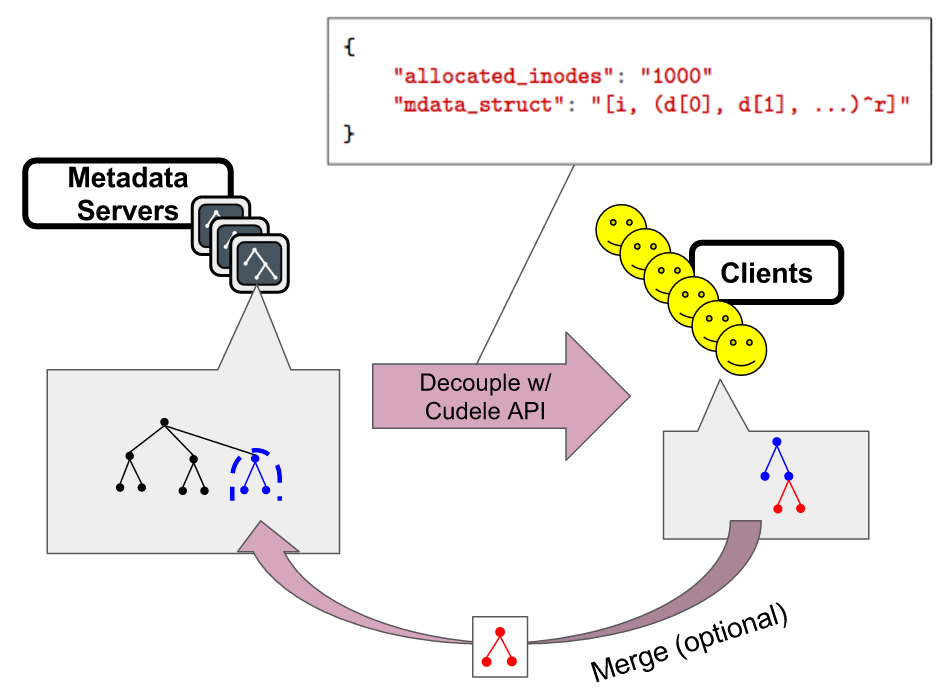
\includegraphics[width=90mm]{figures/arch.png} 
  \caption{System XX lets clients optimize performance by telling the storage
  system about the workload. Clients can specify a Structured Namespace (blue
  subtrees and Section~\ref{sec:structured-namespaces}) or by merging file system
  metadata from an Unstructured Namespace (red subtree and
  Section~\ref{sec:unstructured-namespaces}).}\label{fig:arch}
\end{figure}

% What is Cudele
Cudele is a file system with programmable consistency and durability. Clients
use an API to decouple existing subtrees from the global namespace; metadata
operations from the other clients targeted at the decoupled subtree can be
programmed to be blocked or marked as overwritable. With the decoupled subtree
in hand, the client can do metadata operations locally. Upon completion, the
client can merge the subtree back into the global namespace. 

% Why Cudele is a good fit for implied namespaces
Cudele has the mechanisms for understanding the file system metadata language
and adapting to the workload.  Figure~\ref{fig:arch} shows how clients decouple
the namespace with the Cudele API, specifying how many extra inodes they want
and the structure for the namespace they intend to create. The metadata server
and client both know about the metadata in the blue subtree, requiring no RPCs,
and if the client creates more metadata (red subtree), it can merge it back
into the global namespace.  This model lets users enjoy the simplicity of
global namespaces and the high performance of node-local operations.  We extend
the API to support the declaration of structured namespaces and leverage the
existing API to merge unstructured namespaces. 

\subsubsection{Structured Namespaces}
\label{sec:structured-namespaces}

% What is a structured namespace
A structured namespace is created according to a pattern. If both the client
and metadata server knows the pattern, they can create the metadata
independently. This has two benefits: (1) it reduces RPCs which improves
performance and reduces network traffic and (2) it allows the client and server
to operate in parallel.  The patterns that Cudele understands are shown in
Listing~\ref{src:example} and the programmable interfaces are shown below.
There are two parameters for unstructured namespaces: \texttt{pattern} and
\texttt{trigger}. 

\subsubsection{Trigger: Start Namespace Construction}

% How does trigger work and why do we neet it
\texttt{trigger} specifies when to start the namespace construction on the
metadata server.  The metadata reconstruction can be asynchronous and saving
this resource intense process for later can have better performance. To
facilitate the exploration of different trigger policies, we make the value for
the \texttt{trigger} parameter programmable.  Administrators inject Lua code
that specifies or calculates thresholds for when to start namespace
construction. Although we make this programmable, we do not make any
conclusions about the best trigger time and leave the exploration of this space
as future work.

% example
In Listing~\ref{src:example}, the trigger is:
\begin{listing}
\begin{minted}[frame=single,
               framesep=2mm,
               xleftmargin=10pt,
               tabsize=2]{lua}
{
  if MDSs[whoami]["cpu"] > 30
}
\end{minted}
\label{src:thresh}
\end{listing}

which means that construction of the namespace will start if current MDS
(\texttt{whoami}) has a CPU utilization (\texttt{``cpu"}) above 30\%.

% Drawbacks: consistency
Triggering construction asynchronously can improve performance because the
process can be deferred until the system has less load. However, this
performance gain comes at the cost of consistency. Even if the construction is
triggered immediately, the metadata is eventually consistent; other clients see
outdated metadata because the namespace is sitting on the client. Delaying the
trigger improves the liklihood that system finds a window of low load but also
increases the latency of other clients.\\

\noindent\textbf{Implementation}: we re-use the polling and embedded Lua
virtual machine in Mantle~\cite{sevilla:sc15-mantle} to implement the trigger
interface. By default, every 10 seconds the metadata server checks if the
condition for triggering is satisfied by executing the Lua code. Mantle has
variables exposed for administrators to explore load balancing policies; just
like this work, some of these policies need to identify overloaded metadata
servers so we re-use all those variables.  Some of the more useful variables
include:

\begin{itemize}
  \item Memory Usage
  \item CPU Utilization
  \item Request Rate
  \item Queue Depth
  \item Server Tags: whoami, i
\end{itemize}

\subsubsection{Pattern: Express Namespace}
\label{sec:pattern-express-namespace}

% How does pattern work and why do we need it
\texttt{pattern} describes the metadata layout of the Structured Namespaces. It
is the same language used in~\cite{he:hpdc13-plfs-patterns}. When the metadata
server starts a namespace construction, it creates all the file system metadata
generated by this formula. As a refresher, the pattern in Listing~\ref{src:example}:

  \[[i, (d[0], d[1], ...)^r]\]

means that there are \(r\) entries in the PLFS index file, where the first
entry has a physical offset of \(i\) and lengths of \(d\), where the pattern in
\(d\) repeats. \\

% WTF -- this doesn't give file system metadata! ARGGGGG is it file creations
% or index files shit?

% Drawbacks

\noindent\textbf{Implementation}: Another big fat TODO.

\begin{listing}
\begin{minted}[frame=single,
               framesep=2mm,
               xleftmargin=10pt,
               tabsize=2]{js}
{
  <!-- Structured Namespace Pattern !-->
  "S_pattern": "[i, (d[0], d[1], ...)^r]",
  
  <!-- Structured Namespace Trigger !-->
  "S_trigger": "if MDSs[whoami]["cpu"] > 30",
  
  <!-- Untructured Namespace Allocated Inos !-->
  "US_alloci": "1000",
}
\end{minted}
\caption{Using the Cudele API to express metadata structure, which is
understood by both the server and client.}
\label{src:example}
\end{listing}

\subsubsection{Unstructured Namespaces}
\label{sec:unstructured-namespaces}

\subsubsection{Migrating Metadata Construction}
\label{sec:migrating-metadata-construction}



\bibliographystyle{ACM-Reference-Format}
\bibliography{paper} 

\end{document}
